
\section{targets.xml}

The process file is used to define production and degradation constraints,
i.e. fluxes of metabolic \species{} or \macromolecule{}s that must be maintained
for the cell to be functional.
Constraints can be specified as target fluxes or as target concentrations.

\subsection{RBATargets}
\label{sec:rba_targets}

The outermost part of the process file is an instance of class
\rbatargets, shown in Figure~\ref{fig:targets_doc}.

\begin{figure}
  \centering
  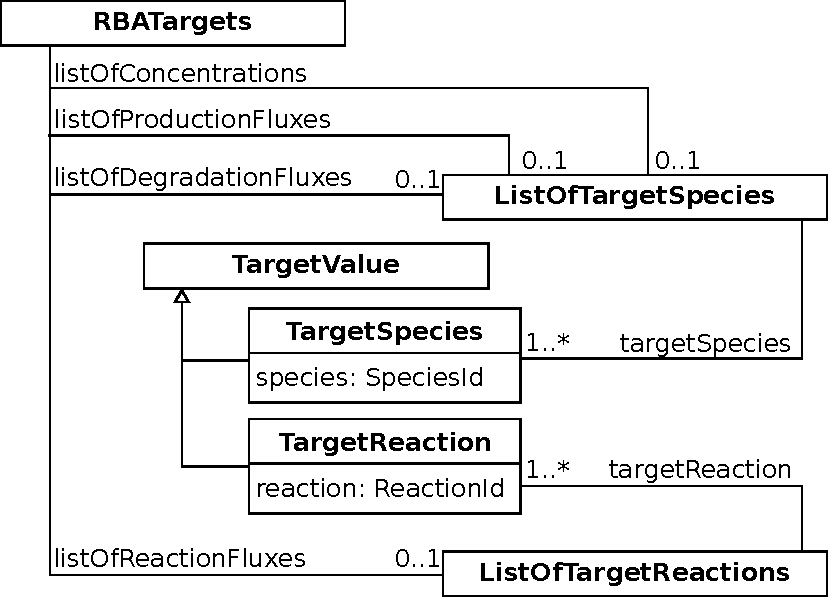
\includegraphics[scale=0.8]{figures/targets_doc}
  \caption{XML structure of target document.}
\label{fig:targets_doc}
\end{figure}

\rbatargets{} has no simple attributes.
It contains 3 \textbf{ListOfTargetSpecies}.
These targets allow to define metabolic \species{} or \macromolecule{} fluxes.
One is for production fluxes, another for degradation fluxes.
The last list is for maintaining a target at a given concentration.
The difference with a simple production flux is that keeping a target at a
concentration depends on growth rate.
More precisely, the flux needed to keep the concentration is
the growth rate multiplied by the target concentration.
Note that all fluxes must be positive.
If the target is a \macromolecule, production/degradation can only occur
if the \processings{} section of some \process{} defines how the
\macromolecule{} is actually produced/degraded.

It contains a \textbf{ListOfTargetReactions}.
It is also possible to define target fluxes as reaction fluxes.
These targets add constraints on the flux of a specific metabolic \reaction.
In this case, fluxes may be positive or negative.


\subsection{TargetSpecies}
\label{sec:target_species}

The \targetspecies{} class defines constraints for a species flux
(Fig.~\ref{fig:targets_doc}).
It inherits \targetvalue{} for the constraint definition part, allowing for
equality or inequality constraints.

\paragraph{The \textit{species} attribute}
The \textbf{species} attribute is a string that must match the identifier
of a metabolic \species{} or a \macromolecule{}.
Note that the \macromolecule{} must be broken down into metabolite costs
through the \processings{} section of some \process{}.
Otherwise no cost will be applied.


\subsection{TargetReaction}
\label{sec:target_reaction}

The \targetreaction{} class defines constraints for a reaction flux
(Fig.~\ref{fig:targets_doc}).
It inherits \targetvalue{} for the constraint definition part, allowing for
equality or inequality constraints.

\paragraph{The \textit{reaction} attribute}
The \textbf{reaction} attribute is a string that must match the identifier
of a metabolic \reaction{}.
